\documentclass[preview]{standalone}

\usepackage{amsmath}
\usepackage{amssymb}
\usepackage{bettelini}
\usepackage{stellar}
\usepackage{chemfig}
\usepackage{tikz}

\hypersetup{
    colorlinks=true,
    linkcolor=black,
    urlcolor=blue,
    pdftitle={Chimica},
    pdfpagemode=FullScreen,
}

\begin{document}

\title{Chimica}
\id{chimica-legami}
\genpage

\section{Energy levels}

\begin{snippet}{energy-levels-explanation}
An electron is a fundamental particle. It is attracted by protons in the
atom nuclei but they repelled by one another.
The places where the electrons are found around the nuclei are called
\textit{atomic orbitals.} \\
There are two types of orbitals, \textbf{s} and \textbf{p}.
Electrons in \textbf{s} orbitals can be measured to be in a spherical region around the nuclei,
whilst electrons in \textbf{p} orbitals have a dumbell-shaped position region
(zero-probability of being measured at the center of the nuclei).
An orbital can host up to two electrons.
Orbitals are grouped in different zones.
Eletrons in zones closer to the center have lower energy and the amount of energy
to move an electron from its zone to the next one is constant.

At the lower energy there is a single \(1\text{s}\) orbital that can hold two electrons.
At the next energy level, there are four orbitals:
\(2\text{s}\), \(2\text{p}1\), \(2\text{p}2\) and \(2\text{s}3\) for up to 8 electrons at this level of energy.
In larger atoms electrons can be found at the level \(3\text{s}\) and \(3\text{p}\)

Atoms where the level with most energy is not completely empty or completely full is unstable.
The excess electrons are called valence electrons. An atom may share, give, or take electrons
with other atoms to become stable.
\end{snippet}

\section{Bonds}

\begin{snippetdefinition}{ionic-bond-definition}{Ionic bond}
    An \textit{ionic bond} is a transfer of valence electrons between metallic atoms and non-metallic atoms.
    The outcome of this process is a positive ion (more protons than electrons)
    and a negative ion (more electrons than protons). These ions attract each other, often
    forming a crystal structure.
\end{snippetdefinition}

\begin{snippetdefinition}{metallic-bond-definition}{Metallic bond}
    A \textit{metallic bond} is a transfer of valence electrons between metallic atoms.
    The valence electrons continually move from one atom to another and are not
    associated with any specific pair of atoms. This creates a structure of positive ions
    that conducts electricity (since electrons can freely move).
\end{snippetdefinition}

\begin{snippetdefinition}{covalent-bond-definition}{Covalent bond}
    A \textit{covalent bond} is a sharing of pairs of electrons between non-metallic atoms.
    A covalent bond happens just between two atoms, it can be simple, double or triple (2, 4, 6 total shared electrons).
\end{snippetdefinition}

\section{Electronegativity}

\begin{snippetdefinition}{electronegativity-definition}{Electronegativity}
    \textit{Electronegativity} is a measure of an atom's ability to attract shared electrons to itself.
    The type of bond is given by the different of electronegativity between two atoms.
\end{snippetdefinition}

\begin{snippet}{elettronegativita-illustration}
    \begin{center}
        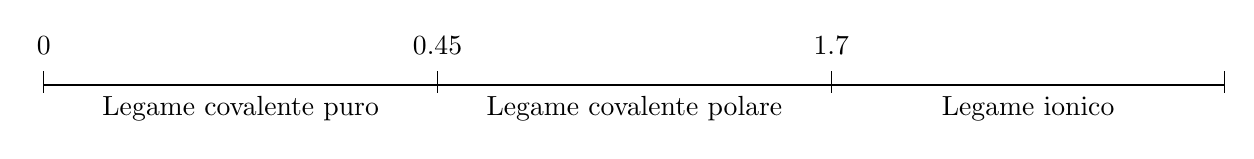
\begin{tikzpicture}
            \draw[thick, -] (0,0) -- (15,0);
            \draw (0 cm, 5pt) -- (0 cm, -3pt);
            \draw (5 cm, 5pt) -- (5 cm, -3pt);
            \draw (10 cm, 5pt) -- (10 cm, -3pt);
            \draw (15 cm, 5pt) -- (15 cm, -3pt);
        
            \node at (0, 0.5) {0};
            \node at (5, 0.5) {0.45};
            \node at (10, 0.5) {1.7};
            \node at (2.5, -0.3) {Legame covalente puro};
            \node at (7.5, -0.3) {Legame covalente polare};
            \node at (12.5, -0.3) {Legame ionico};
        \end{tikzpicture}
    \end{center}
\end{snippet}

\section{Simboloia di Lewis}

\begin{snippet}{simbologia-lewis-expl}
    La simbologia di Lewis è un metodo grafico per rappresentare la formazione dei legami chimici.
    Questa notazione proietta gli elettroni del guscio più esterno, dunque quelli coinvolti nella
    formazione dei legami, attraverso puntini disposti intorno al simbolo dell'elemento.
    Una doppietta di elettroni non accoppiati possono essere indicati anche come una riga.
    \\
    \begin{center}
        \fbox{
            \chemfig{\Charge{0=\.}{Li}} \quad
            \chemfig{\Charge{0=\.,180=\.}{Be}} \quad
            \chemfig{\Charge{0=\.,180=\.,90=\.}{B}} \quad
            \chemfig{\Charge{0=\.,180=\.,90=\.,-90=\.}{C}} \quad
            \chemfig{\Charge{0=\.,180=\.,90=\|,-90=\.}{N}} \quad
            \chemfig{\Charge{0=\.,180=\.,90=\|,-90=\|}{O}} \quad
            \chemfig{\Charge{0=\|,180=\.,90=\|,-90=\|}{F}} \quad
            \chemfig{\Charge{90=\|,0=\|,-90=\|,180=\|}{Ne}}
        }
    \end{center}
\end{snippet}

\plain{<br>}

\end{document}
